% This file was created by matplotlib2tikz v0.7.4.
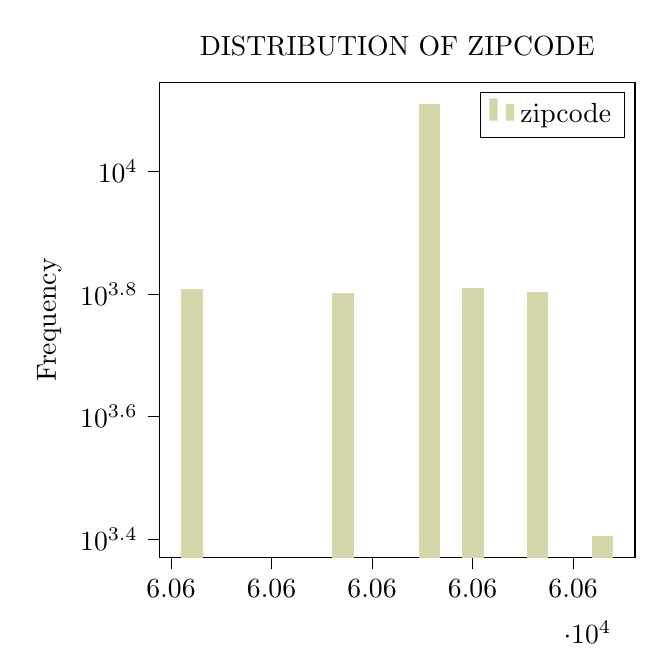
\begin{tikzpicture}

\definecolor{color0}{rgb}{0.835294117647059,0.83921568627451,0.666666666666667}

\begin{axis}[
height=3in,
log basis y={10},
tick align=outside,
tick pos=left,
title={\printsubsection{\MakeUppercase{Distribution of zipcode}}\\},
width=3in,
x grid style={white!69.01960784313725!black},
xmin=60598.85, xmax=60646.15,
xtick style={color=black},
y grid style={white!69.01960784313725!black},
ylabel={Frequency},
ymin=2341.74275213975, ymax=13996.4818808774,
ymode=log,
ytick style={color=black}
]
\draw[fill=color0,draw opacity=0] (axis cs:60601,0) rectangle (axis cs:60603.15,6427);
\addlegendimage{ybar,ybar legend,fill=color0,draw opacity=0};
\addlegendentry{zipcode}

\draw[fill=color0,draw opacity=0] (axis cs:60603.15,0) rectangle (axis cs:60605.3,0);
\draw[fill=color0,draw opacity=0] (axis cs:60605.3,0) rectangle (axis cs:60607.45,0);
\draw[fill=color0,draw opacity=0] (axis cs:60607.45,0) rectangle (axis cs:60609.6,0);
\draw[fill=color0,draw opacity=0] (axis cs:60609.6,0) rectangle (axis cs:60611.75,0);
\draw[fill=color0,draw opacity=0] (axis cs:60611.75,0) rectangle (axis cs:60613.9,0);
\draw[fill=color0,draw opacity=0] (axis cs:60613.9,0) rectangle (axis cs:60616.05,0);
\draw[fill=color0,draw opacity=0] (axis cs:60616.05,0) rectangle (axis cs:60618.2,6332);
\draw[fill=color0,draw opacity=0] (axis cs:60618.2,0) rectangle (axis cs:60620.35,0);
\draw[fill=color0,draw opacity=0] (axis cs:60620.35,0) rectangle (axis cs:60622.5,0);
\draw[fill=color0,draw opacity=0] (axis cs:60622.5,0) rectangle (axis cs:60624.65,0);
\draw[fill=color0,draw opacity=0] (axis cs:60624.65,0) rectangle (axis cs:60626.8,12904);
\draw[fill=color0,draw opacity=0] (axis cs:60626.8,0) rectangle (axis cs:60628.95,0);
\draw[fill=color0,draw opacity=0] (axis cs:60628.95,0) rectangle (axis cs:60631.1,6459);
\draw[fill=color0,draw opacity=0] (axis cs:60631.1,0) rectangle (axis cs:60633.25,0);
\draw[fill=color0,draw opacity=0] (axis cs:60633.25,0) rectangle (axis cs:60635.4,0);
\draw[fill=color0,draw opacity=0] (axis cs:60635.4,0) rectangle (axis cs:60637.55,6354);
\draw[fill=color0,draw opacity=0] (axis cs:60637.55,0) rectangle (axis cs:60639.7,0);
\draw[fill=color0,draw opacity=0] (axis cs:60639.7,0) rectangle (axis cs:60641.85,0);
\draw[fill=color0,draw opacity=0] (axis cs:60641.85,0) rectangle (axis cs:60644,2540);
\end{axis}

\end{tikzpicture}